\chapter{I Asked Miami Millionaires How They Got Rich}

This lecture is not mathematical in the narrow blackboard sense, but it is quantitative all the way through. We are first shown outputs---a private jet, a Lamborghini, eight-figure exits, a reported annual income near \text{\$}2 million, a business doing \text{\$}5.5 million gross and \text{\$}2.4 million net, and finally a year at \text{\$}752 million in revenue---and only afterward are we allowed to ask what operating rules might generate such scales. The proper way to read the chapter, then, is as a sequence of commercial models: producer versus consumer, gross versus net, speed versus delay, cash flow versus asset accumulation, and rich versus free.

No validated mathematical frame survives from the video, so every formal relation below is transcript-backed or a cautious reconstruction. We therefore keep especially close to the order of the narration. The host opens with spectacle, then turns that spectacle into a field study of Miami wealth, and only then begins to extract definitions, mechanisms, and update rules from one interview after another.

\section{Opening Montage: Wealth First, Explanation Later}

The cold open is deliberately structured as an inverse problem. We see wealth before we are told how it was built. A private jet is followed by the claim of two tech companies run for roughly ten years and sold for eight figures. Another clip gives a migration story beginning with \text{\$}78 in cash and ending at about \text{\$}2 million annually. A third reports \text{\$}5.5 million gross and \text{\$}2.4 million net. A fourth reaches a year at \text{\$}752 million in revenue. The host then asks the right question: how can somebody own a private jet in today's world?

The scene widens into Miami itself. The city is introduced as home to nearly forty thousand millionaires, and the lecture promises to convert visual wealth into practical commercial method:
\begin{align}
M_{\mathrm{Miami}} &\approx 4\times 10^4,\\
I_{\mathrm{annual}} &\approx \text{\$}2\,\mathrm{M},\\
G &= \text{\$}5.5\,\mathrm{M}, \qquad N = \text{\$}2.4\,\mathrm{M},\\
R_{2023} &= \text{\$}752\,\mathrm{M}.
\end{align}

\begin{remark}
These are reported figures, not audited data. Their role in the lecture is motivational and structural: they set the scale of the problem we are about to study.
\end{remark}

At this point the chapter must resist a common mistake. The opening is not disposable montage. It is the lecture's first piece of pedagogy. We are meant to feel the distance between the visible endpoint and the still-hidden mechanism. That distance is what the interviews will spend the rest of the chapter closing.

\section{From Broke to Producer Logic}

The first full interview begins where many of these conversations begin: with broke-ness. The speaker recalls sleeping in a car, lacking money altogether, and growing up under severe material limitation. But the real work of the segment begins only after credibility has been established through hardship. The lecture then pivots to classification.

\begin{definition}
In the local language of the lecture, a \emph{consumer} stands on the side of consuming existing value, while a \emph{producer} stands on the side of creating and offering value. The buyer-seller distinction is used as a practical restatement of the same divide.
\end{definition}

\begin{proposition}
Within the lecture's simplified commercial picture, durable monetary capture lies closer to the producing and selling side of exchange than to the consuming and buying side.
\end{proposition}

\begin{proof}
Consumers move money outward in order to obtain a good, service, or solution. Producers and sellers receive money in exchange for what they create, organize, or distribute. Thus, if we ask where accumulation begins, the lecture places the answer on the producing side of the transaction.
\end{proof}

The claim can be summarized schematically as
\begin{equation}
\mathrm{Income}(\text{producer}) > \mathrm{Income}(\text{consumer}),
\qquad
\mathrm{ValueCapture}(\text{seller}) > \mathrm{ValueCapture}(\text{buyer}).
\end{equation}
We should not misread this as a universal theorem. It is a rule of orientation. The lecture is telling us where to stand in the stream of exchange if we want money to flow toward us rather than away from us.

\subsection{Question \& Answer}

\paragraph{Question.} Are you a buyer or a seller?

\paragraph{Answer.} The speaker answers: seller. He then generalizes the answer into a broader pair, consumer and producer. Selling, in this account, is not merely a tactic. It is a position inside the exchange. To buy is to spend in order to receive; to sell is to organize what others will pay for.

\begin{figure}[h]
\centering
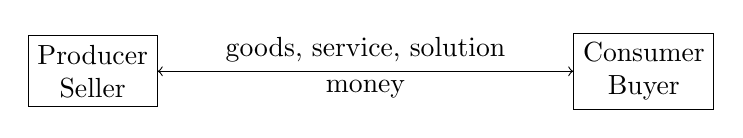
\begin{tikzpicture}
\node[draw, align=center] (p) at (0,0) {Producer\\Seller};
\node[draw, align=center] (c) at (7,0) {Consumer\\Buyer};
\draw[->] (p) -- node[above] {goods, service, solution} (c);
\draw[->] (c) -- node[below] {money} (p);
\end{tikzpicture}
\end{figure}

The lecture does not stop with this first distinction. The same speaker immediately adds three loves that must accompany producer logic: people, sales, and numbers. This is important. Pure abstraction is not enough. We must be able to deal with human beings, move an offer through language, and keep accurate account. From there the segment accelerates outward into speed, anti-procrastination, giving rather than taking, and the injunction to work with the whole person while still recognizing that no individual is all-powerful. The interview ends in the host's own key phrase: the classification was good, but it becomes useful only once it is turned into disciplined practice.

\section{Tech, Exits, and the Value of Speed}

The next segment brings the same problem into the startup world. The speaker says he grew up in the tech business, ran two tech companies for about ten years, sold both, and now enjoys life in Miami after eight-figure exits. The host then asks the operational question: how does one break into tech in 2024?

The answer is built around timing. A good idea today may be duplicated tomorrow. That means the key interval is not simply invention, but the time between idea and market:
\begin{equation}
\Delta t_{\mathrm{idea}\to\mathrm{market}} \downarrow
\quad \Longrightarrow \quad
\text{imitation risk before capture} \downarrow .
\end{equation}
This is not a measured law, but it is exactly the structure of the speaker's argument. In markets where replication is fast, execution speed becomes a source of economic advantage.

The lecture then supplies the supports that make such speed possible. First come great people: smart, committed people who actually want to work inside the strain of a startup. Second comes capitalization. The speaker does not merely say ``money''; he says ``smart money.'' That phrase matters. Capital here is not treated as a passive pile of funds but as informed fuel: judgment, runway, discipline, and network carried inside the financing itself.

The lecture's local conclusion is simple and sharp. If one asks what field is most alive in 2024, the answer given is tech, and more narrowly AI. The host then performs one of his typical recap transitions. He compresses the interview into a portable lesson: go fast, yes, but understand that the thing making speed possible is the quality of the people around you. This recap is pedagogically important, because it carries one interview's result directly into the next.

\section{Freedom, Complaint, and the Refusal of Entitlement}

The tone changes here, but the structure does not. We are again asked about being broke, and again the answer is quantitative and narrative at once. The speaker says she came to the United States with \text{\$}78 in cash, did not speak English, and now makes about \text{\$}2 million annually:
\begin{equation}
M_0 = \text{\$}78,
\qquad
I_{\mathrm{annual}} \approx \text{\$}2\,\mathrm{M}.
\end{equation}

\begin{remark}
The first quantity is an initial stock; the second is a later annual flow. The lecture uses the contrast narratively, not as part of a formal compound-growth calculation.
\end{remark}

What is new in this beat is the stated end. The favorite part of being a business owner in the United States is not luxury but freedom. Money is therefore not the terminal object. It is a means by which poverty is not repeated onto the next generation.

The host then asks a stronger question than biography alone can answer: what do successful people have in common? The reply is not genius, pedigree, or exceptional circumstances. It is that they do not complain. They stay on the side of solution. They do not sit in self-pity. They ask, instead, what can be done better. That answer is then sharpened further. Entitlement, the speaker says, is what kills you. Nobody is coming to save you.

The final turn of the segment is about noise. If we listen to people who do not have what we want, we inherit their limits. In the speaker's own example, others dismissed the chosen business as strange or unserious. The result came not from consensus but from obsessive improvement in the craft itself. The host's recap is faithful to the flow of the lecture: do not complain, do not feel entitled, and do not confuse outside opinion with a binding law of outcomes.

\section{Gross, Net, Failure, and Accountability}

We now arrive at the densest operational segment in the chapter. A young entrepreneur in a Lamborghini describes a main marketing agency feeding other companies, a time horizon of roughly twenty-two months, and a first full year at \text{\$}5.5 million gross but \text{\$}2.4 million net:
\begin{align}
G &= \text{\$}5.5\,\mathrm{M},\\
N &= \text{\$}2.4\,\mathrm{M},\\
N &= G - K.
\end{align}
Here \(K\) is the total subtraction between top line and retained result: costs, operating expense, and all the leak between visible scale and actual keep. The speaker's emphasis is unambiguous: the net figure is what matters.

\paragraph{Worked Example.}
The transcript gives us just enough to do a disciplined piece of arithmetic.
\begin{enumerate}
\item Begin with the reported top line and retained result:
\[
G=\text{\$}5.5\,\mathrm{M},
\qquad
N=\text{\$}2.4\,\mathrm{M}.
\]
\item Infer the residual cost bucket:
\[
K = G-N = \text{\$}3.1\,\mathrm{M}.
\]
\item Compute the retained fraction of gross:
\[
\frac{N}{G} \approx \frac{2.4}{5.5} \approx 0.436.
\]
\item Hence about \(43.6\%\) of the reported gross survives into the figure the speaker explicitly values, while the remaining \(56.4\%\) is absorbed by the machinery of operating at that scale.
\end{enumerate}
The lecture's lesson is not anti-growth. It is anti-illusion. A large top line is weaker than it appears if very little of it remains.

The same speaker then recounts a chain of collapses and resets: an early clothing store and barbershop, failure through bad partnership conditions, restarting with phone sales, losses in real estate, and finally a move into insurance because it appeared to offer an uncapped or at least unusually open earning structure. The lecture does not present this as glamorous. It presents it as the reality of serial adjustment.

\subsection{Question \& Answer}

\paragraph{Question.} What keeps people broke?

\paragraph{Answer.} The strongest answer in the segment is that events need not be your fault in order to become your problem. Once something is your problem, failure to solve it is what perpetuates brokenness. The lecture then names concrete bottlenecks: money management, time management, and the refusal to prospect.

That final point can be written as an operational chain:
\begin{equation}
P_t \uparrow \Rightarrow L_t \uparrow \Rightarrow S_t \uparrow,
\end{equation}
where \(P_t\) denotes prospecting effort, \(L_t\) the stock of active relationships or live conversations, and \(S_t\) realized sales. Talent in selling does not monetize in a vacuum. It monetizes only after prospecting has produced opportunities on which talent can act.

A second chain, more psychological but still practical, is also implied:
\begin{equation}
B_t \uparrow \Rightarrow W_t \uparrow \Rightarrow P_t \uparrow,
\end{equation}
where \(B_t\) stands for belief in oneself and \(W_t\) for work intensity. Again, this is not psychometrics. It is a local causal order: weak belief lowers work, lowered work reduces prospecting, and weak prospecting starves sales.

The host's recap after this beat is especially clean. He repeats the large outcome, but he does not let the outcome dominate the lesson. The lesson is accountability: whether or not the original blow was ours to blame, solving it is still ours to do.

\section{Cash Flow as the Engine of Asset Growth}

The mansion interview finally turns us from earning into deployment. An orthodontist says he has made multiple millions and pushed money into shopping centers and other real-estate assets. The host asks exactly the right question: what is the secret of creating wealth in real estate, especially given the widespread belief that one must begin with a ton of money?

\subsection{Question \& Answer}

\paragraph{Question.} How do we create wealth in real estate without starting with a ton of money?

\paragraph{Answer.} The answer is recursive. We first grow a core practice. That practice throws off cash flow. We then use that cash flow to buy shopping centers or medical buildings. Those assets then generate further cash flow. The next cycle begins from a larger base than the previous one.

In cautious notation,
\begin{align}
C_{t+1} &= C_t^{\mathrm{practice}} + C_t^{\mathrm{asset}},\\
A_{t+1} &= A_t + \Delta A(C_t).
\end{align}
The first line says that next-period deployable cash is the sum of cash from the operating practice and cash from already acquired assets. The second says that the asset stock grows by whatever new purchases current cash flow can support.

\begin{figure}[h]
\centering
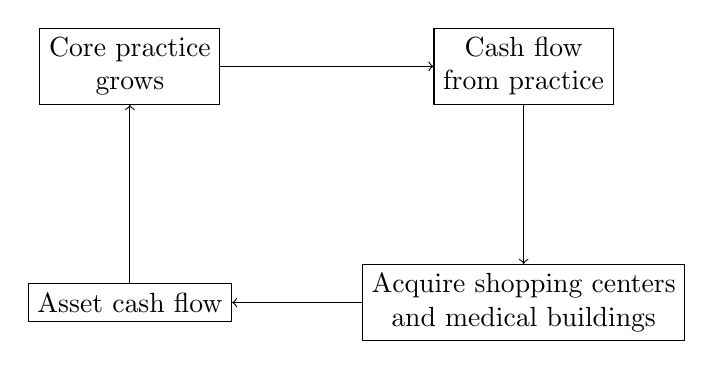
\begin{tikzpicture}
\node[draw, align=center] (practice) at (0,0) {Core practice\\grows};
\node[draw, align=center] (cash) at (5,0) {Cash flow\\from practice};
\node[draw, align=center] (buy) at (5,-3) {Acquire shopping centers\\and medical buildings};
\node[draw, align=center] (asset) at (0,-3) {Asset cash flow};
\draw[->] (practice) -- (cash);
\draw[->] (cash) -- (buy);
\draw[->] (buy) -- (asset);
\draw[->] (asset) -- (practice);
\end{tikzpicture}
\end{figure}

This is the clearest compounding mechanism in the lecture. We do not need leverage formulas, cap rates, or discount factors to follow it. The business generates cash, cash buys assets, assets generate more cash, and the process repeats.

The speaker then adds two necessary correctives. First, certain core businesses come with high barriers to entry. In his own case, dental school and orthodontic training took eleven years. Second, real estate is not purely mechanical. Access to deals depends on being directly in front of owners and being the sort of person with whom they want to transact. Thus even this most financial-looking loop still rests on social friction and human trust.

\section{Feeding the Business, Building Sustainability, and Selling at Scale}

The final interview is the capstone. The scale rises: thirty years in business, tens of millions in yearly earnings, \text{\$}100 million exits, and a best year at
\begin{equation}
R_{2023} = \text{\$}752\,\mathrm{M}.
\end{equation}
But the lecture once again refuses to stop at the number. What matters is what this scale licenses the speaker to say.

The first rule is epistemic: ask questions. The speaker is almost astonished that people will stand in a room with someone operating at a higher level and remain silent. Curiosity is treated here not as ornament but as an accelerant. If one wants compression of learning, one asks relentlessly.

\subsection{Question \& Answer}

\paragraph{Question.} What is the best financial advice for building a sustainable business?

\paragraph{Answer.} Two answers are layered together. First, feed the business rather than starving it. If margins are small and time to scale is long, the firm must remain resourced until its eventual economics have room to appear. Second, evaluate decisions through what the speaker calls a three-legged stool: the customer, the worker side, and the company itself must all remain intact.

Schematically, the second rule can be written as
\begin{equation}
D\ \text{admissible}
\iff
E_{\mathrm{cust}}(D)\ge 0,\ 
E_{\mathrm{team}}(D)\ge 0,\ 
E_{\mathrm{firm}}(D)\ge 0.
\end{equation}
Here \(D\) is a business decision, and the \(E\)'s are its effects on customer, team, and firm. This is not the lecture's literal wording, but it preserves the architecture exactly: if one leg fails, the stool is unstable.

\begin{figure}[h]
\centering
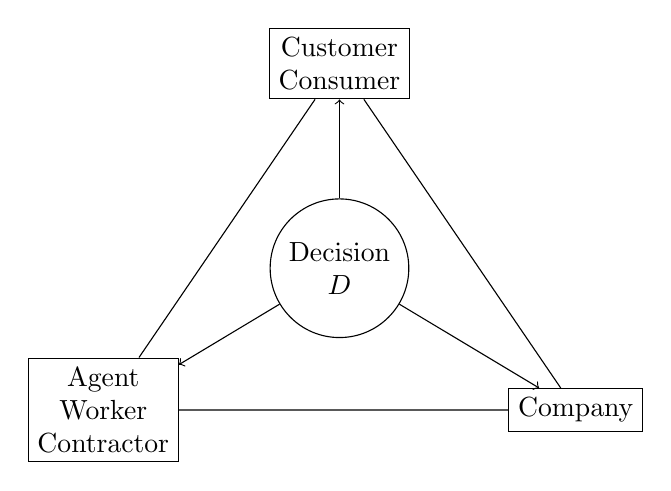
\begin{tikzpicture}
\node[draw, align=center] (top) at (0,2.6) {Customer\\Consumer};
\node[draw, align=center] (left) at (-3,-1.8) {Agent\\Worker\\Contractor};
\node[draw, align=center] (right) at (3,-1.8) {Company};
\node[draw, circle, align=center] (center) at (0,0) {Decision\\\(D\)};
\draw[->] (center) -- (top);
\draw[->] (center) -- (left);
\draw[->] (center) -- (right);
\draw (top) -- (left) -- (right) -- (top);
\end{tikzpicture}
\end{figure}

The lecture then introduces one of its most important distinctions: not everybody enters business to get the same thing. Many, says the speaker, enter to get rich right away. He entered to get free, believing that wealth would come later. This is not sentimental language. It is a capital-withdrawal rule. Pull out too early and one may look rich while remaining weak; feed the business long enough and one may look poorer while becoming durable.

The closing movement of the segment turns to sales. Why do people fail at it? Because, says the speaker, they do not believe in themselves, and without belief they do not work hard enough. His own method is extremely behavioral: call more people, do not fear judgment, refuse to stop at the first no, and recognize that the market is less competitive than it appears because so many people will not sustain the labor.

We can collect this into one last schematic chain:
\begin{equation}
B_t \uparrow \Rightarrow W_t \uparrow \Rightarrow P_t \uparrow \Rightarrow L_t \uparrow \Rightarrow S_t \uparrow.
\end{equation}
Belief raises work, work raises prospecting, prospecting raises the number of live relationships, and those relationships create the occasions in which sales can actually occur. The lecture is careful here. Sales skill matters, but it is downstream of discipline.

That is why the segment ends not with abstract positivity but with a harder rule: the first rule of business is to stay in business. Patience is not passivity. It is a design condition for survivability.

\section{Summary}

The chapter opens with spectacle but earns its seriousness by moving steadily toward structure. Its strongest distinctions are the ones we should keep: producer versus consumer, buyer versus seller, gross versus net, complaint versus solution, rich versus free. Around those distinctions the lecture organizes a set of practical update rules. Speed matters in tech because imitation arrives quickly. Cash flow matters in real estate because it can be turned into asset stock, and asset stock can return to cash flow. Prospecting matters in sales because talent without contact remains inert. Patience matters in business because a company must be fed before it can carry us.

Nothing here should be overstated. These are not theorems of economics. They are disciplined claims made by operators describing how they believe they built what the opening montage displayed. Still, that is exactly why the lecture is worth preserving. Even where it sounds motivational, it keeps resolving motivation into mechanism. The visible wealth is only the surface. The real content lies in flows, positions, constraints, and repeated loops, and those are the notes we ought to carry forward.